\documentclass[bachelor,german]{hgbthesis}
% Zulässige Class Options: 
%   Typ der Arbeit: diplom, master (default), bachelor, praktikum 
%   Hauptsprache: german (default), english
%%------------------------------------------------------------

\graphicspath{{images/}}    % wo liegen die Bilder? 
\bibliography{literatur}  	% Angabe der BibTeX-Datei, % utf8-change

%%%  Acronym and Glossary
\usepackage[utf8]{inputenc}
\usepackage[acronym, toc]{glossaries}
\makenoidxglossaries

\newglossaryentry{maths}
{
    name=mathematics,
    description={Mathematics is what mathematicians do}
}

\newacronym{lcm}{LCM}{Least Common Multiple}
\newacronym{IoT}{IoT}{Internet of Things}
\newacronym{DAPP}{DAPP}{Decentralized Application}
\newacronym{DAPPs}{DAPPs}{Decentralized Applications}
\newacronym{EVM}{EVM}{Ethereum Virtual Machine}

%%%----------------------------------------------------------
\begin{document}
%%%----------------------------------------------------------

% Einträge für ALLE Arbeiten:
\title{lokkit - Einsatz von Blockchain und IoT}
\author{D.\ Hirzel\ und A.\ Schmid}
\studiengang{Informatik}
\studienort{Rotkreuz}
\abgabedatum{2017}{06}{09}	% {YYYY}{MM}{DD}
%\strictlicense  % erzeugt restriktive Lizenzformel

%%%----------------------------------------------------------
\frontmatter
\maketitle
\tableofcontents
%%%----------------------------------------------------------		

% \include{chapters/02_Selbststaendigkeitserklaerung} wird durch \maketitle bereits gemacht.
\chapter{Abstract d}
\label{cha:abstract_d}

Die \emph{Blockchain}-Technologie ist zurzeit stark im Trend. Sie benutzt verteilte und dezentrale Rechnernetzwerke und bietet dadurch bessere Transparenz und geringere Kosten im Vergleich zu traditionellen Methoden. Auch wird dadurch die Sicherheit erhöht, da die einzelnen Nodes sich gegenseitig versichern, wahrheitsgemäss zu handeln.\cite{BlockchainRevolution}

Pioniert wurde die Blockchain Technologie durch die bekannte bitcoin Blockchain. Neue Blockchain Implementationen unterstützen neben Crypto-Währungen auch sogenannte \emph{Smart Contracts}, die es einem Benutzer erlauben, Programmcode zu implementieren, der in der Blockchain abgelegt wird. Dadurch, dass dieser Code zusammen mit den Daten einsehbar ist, können so Verträge unmissverständlich und öffentlich einsehrbar definiert werden. Programme, die diese Smart Contracts verwenden, nennt man auch \emph{\acrfull{DAPP}}.\cite{BlockchainRevolution}

Auch das Thema \acrshort{IoT} ist seit mehreren Jahren in aller Munde und wächst in den kommenden Jahren stark an. Gartner schätzt einen Zuwachs von 20.4 Milliarden Geräten bis 2020. Dies bringt neue Anforderungen an die Sicherheit mit - ein Aspekt, der eventuell durch die Blockchain-Technologie erfüllt werden kann.\cite{gartner.com_iot,BlockchainRevolution}



\chapter{Abstract d}
\label{cha:abstract_d}

Abstract goes here

%\printglossary[title=Abkürzungen und Definitionen, toctitle=List of terms]

\printnoidxglossary[type=\acronymtype]
 
\printnoidxglossary

%%%----------------------------------------------------------
\mainmatter         % Hauptteil (ab hier arab. Seitenzahlen)
%%%----------------------------------------------------------

\chapter{Aufgabenstellung}
\label{cha:Aufgabenstellung}
\begin{itemize}
    \item \textbf{Grob beschreiben, was erreicht werden soll. Wünsche von Auftraggeber}
    \item \textbf{Eigene Idee und Wünsche erklären. Brainstorming für Ideen auflisten (evtl. Anhang)}
    \item \textbf{lokkit. Konkrete Aufgabenstellung mit use cases, szenarien, business überlegungen (für Hüsler, bspw. möglichen Missbrauch und "kriminelle Energie" erläutern) und requirements. KEINE technischen details, diese folgen im Kapitel Implementation} \ref{sec:Implementation}
    \item \textbf{Erkären warum Wunsch von Auftraggeber erfüllt}
\end{itemize}

Hier folgt die Aufgabenstellung, die ebenfalls im Rahmen dieser Projektarbeit erarbeitet wurde. Einzig die Schlagworte \emph{Blockchain}, \emph{\acrfull{IoT}} und der Bau eines Demonstrators waren vom Auftraggeber im Kick-Off Meeting vorgegeben worden. Im Rahmen dieser Bachelorarbeit sollte ein System definiert, konzipiert und entwickelt werden, das den Blockchain und IoT Aspekt verbindet und einen praktischen Anwendungszweck demonstriert. Der entwickelte Demonstrator sollte nach Abschluss dieses Projektes noch weiter vom Auftraggeber als solcher verwendet werden können.

\section{Ziele}
\label{sec:Ziele}
"Der zentrale Aspekt dieses Projektes war der Wissenserwerb im Bereich Blockchain und die konkrete Anwendung dieses neu erworbenen Wissens durch die Konzeption und Implementation eines IoT Demonstrators. Dieser sollte durch sorgfältige und gründliche Arbeit dem Auftraggeber in einem eigenständig verwendbaren Zustand übergeben werden können. Die konkrete Aufgabenstellung für den Demonstrator wurde ebenfalls im Rahmen dieses Projektes vom Projektteam entwickelt und mit dem Auftraggeber besprochen", \ref{pm_subsec:Projektziele}.

\section{Konkrete Aufgabenstellung}
\label{sec:Konkrete_Aufgabenstellung}
\emph{Da die konkrete Aufgabenstellung in dieser Bachelorarbeit ebenfalls erarbeitet werden musste, ist diese ein Produkt der Recherchephase (vgl. \ref{pm_subsubsec:Recherchephase}). Bei fehlendem Wissen um Blockchain, Ethereum oder den entwickelten Demonstrator wird empfohlen, die einleitenden Kapitel der Lösungsfindung \ref{sec:Arbeitsmethodik} und \ref{sec:Recherche} vorzugreifen.}

Es soll ein System entwickelt werden, um Schliessfächer zu (ver-)mieten. Dabei sollen die Verträge in Form von Smart Contracts (vgl. \ref{subsec:Recherche_Smart_Contracts}) in einer privaten Ethereum Blockchain (vgl. \ref{subsec:private_chain}) definiert werden. Ein Benutzer soll über eine grafische Benutzeroberfläche ein freies Schliessfach reservieren können. Während der Benutzer der aktuelle Mieter eines Faches ist, kann er das Schloss per Knopfdruck ver- und entriegeln.

\section{Anforderungen an den Demonstrator}
\label{sec:Anforderungen_Demonstrator}

\subsection{Smart Contracts}
Die Businesslogik und Datenhaltung ist mittels Smart Contracts zu lösen. Diese bilden das zentrale Objekt in diesem System.

X. Die Smart Contracts sollen eine Funktion bieten, neue Schliessfächer erfassen zu können.

X. Die Smart Contracts sollen eine Funktion zum Eingehen eines zeitlich begrenzten Mietvertrags anbieten.

X. Die Smart Contracts soll Kosten für die Dauer des Mietvertrags definieren, die durch die Überweisung von Ether beglichen werden.

//X. Der Benutzer soll ein Depot für die Mietdauer an die Smart Contracts entrichten, das dem Besitzer eines Schliessfaches als Sicherheit dient, falls das Schliessfach nicht freigegeben wird.

\subsection{Webapp}
Die Interaktion von Benutzern mit Smart Contracts in der Blockchain wird durch eine Webapp umgesetzt. Folgende Anforderungen beziehen sich auf zu entwickelnde Webapp.\cite[Wiki/DAPP-Developer-Resources, Wiki/Useful-Dapp-Patterns]{github.com/ethereum}

X. Die Webapp soll eine Liste von verfügbaren Schliessfächer anzeigen.

X. Die Webapp soll das einfache Hinzufügen von Schliessfächern zu der Liste der verfügbaren Schliessfächern ermöglichen.

X. Die Webapp soll das Mieten von Schliessfächern mit einer einfach zu bedienenden Benutzeroberfläche ermöglichen.

//X. Die Webapp soll dem Benutzer in allen Fällen Rückmeldung über ausgeführte Funktionen geben.

X. Die Webapp soll auf der zur Verfügung gestellten Hardware gehostet werden können (namentlich: Raspi)

\subsection{Mobile App}
Folgende Anforderungen beschränken sich auf die Mobile App für Android (später: Android App).

X. Die Mobile App soll eine Ethereum Node starten, die mit dem definierten privaten Netzwerk verbindet und die verwendet werden, um die Webapp lokal mit der Node zu verbinden.

X. Die Mobile App soll die Erstellung von einem Benutzerkonto auf der lokalen Ethereum Node ermöglichen.

X. Die Mobile App soll...

\subsection{IoT Controller}
Damit die Schliessfächer angesprochen werden können, müssen auf den IoT Geräten Controller implementiert werden, die die Hardware ansteuern. Folgende Anforderungen gelten für alle Controller unterschiedlicher Hardware.

X. Der Controller soll auf gültige Anfragen das Schliessfach öffnen oder schliessen.

\subsection{Demonstrator Hardware}


X. Der Demonstrator soll ohne externe Abhängigkeiten funktionsfähig sein.

X. Der Demonstrator soll...

\subsection{Übergreifend}
Diese Anforderungen sind funktionsübergreifend gültig und müssen von allen betroffenen Komponenten berücksichtigt werden.

X. Ver- und Entriegeln eines Schliessfachs kann nur von einem durch einen Smart Contract berechtigten Benutzer erfolgen.

X. Alle Implementationen mit grafischer Benutzeroberfläche sollen in einem einheitlichen Erscheinungsbild erstellt werden.

\subsection{Scopeabgrenzung}
X. Das Hinzufügen von neuen mietbaren Objekten ist nicht Teil dieser Arbeit. Der Demonstrator wird mit den mitgelieferten Schliessfächern vorkonfigurierten.

X. Die Verwendung von Oracles ist nicht Teil dieses Projekts. Als Oracle wird die Möglichkeit bezeichnet, Berechnungen eines Smart Contracts, durch Verteilung auf mehrere externe Systeme, von der Blockchain zu lösen. Dies ist noch immer ein low-trust Szenario, da keinem externen System alleine die Möglichkeit zur Veränderung der Blockchain gegeben wird, sondern auch der Konsens dieser Systeme in die Blockchain geschrieben wird.\cite{blog.ethereum.org/oracles}

aus einem Smart Conract heraus Systeme anzusprechen, die nicht auf der Blockchain funktionieren. Beispielsweise existieren 

\section{Erwartete Resultate}
\label{sec:Erwartete_Resultate}

\subsection{Software}
\begin{itemize}
    \item Smart Contracts in Solidity
    \item Webapp (Plattformunabhängig)
    \item Mobile App (Android exkl.)
    \item IoT Controllers
\end{itemize}

\subsection{Hardware}
\begin{itemize}
    \item Ein lauffähiger Demonstrator für das Schliessfachsystem.
\end{itemize}

\chapter{Lösungsentwicklung}
\label{cha:Lösungsentwicklung}
Um eine Lösung zu dieser 

\section{Arbeitsmethodik}
Da in diesem Projekt eine konkrete Aufgabenstellung selbst zu erarbeiten war, und keine konkreten, lieferbaren Objekte vorgesehen waren, wurde zu Beginn eine explorative ad-hoc Methodik verfolgt. Dabei wurde im Projektteam wöchentlich der bisherige Fortschritt analysiert und weitergehende Schritte besprochen. So wurde gewährleistet, dass in der Anfangsphase eine geeignete Aufgabenstellung gefunden werden kann.
\par
Sobald die Aufgabenstellung gefunden wurde, wurde in ein iterativ- inkrementelles Modell gewechselt. Die wöchentlichen Besprechungen wurden beibehalten, um den Fortschritt des Produkts zu verfolgen.

\section{Systemübersicht IoT}
\label{sec:Setup_IoT}
Übersicht: Raspis, Schliessfächer etc...
\begin{figure}
\centering
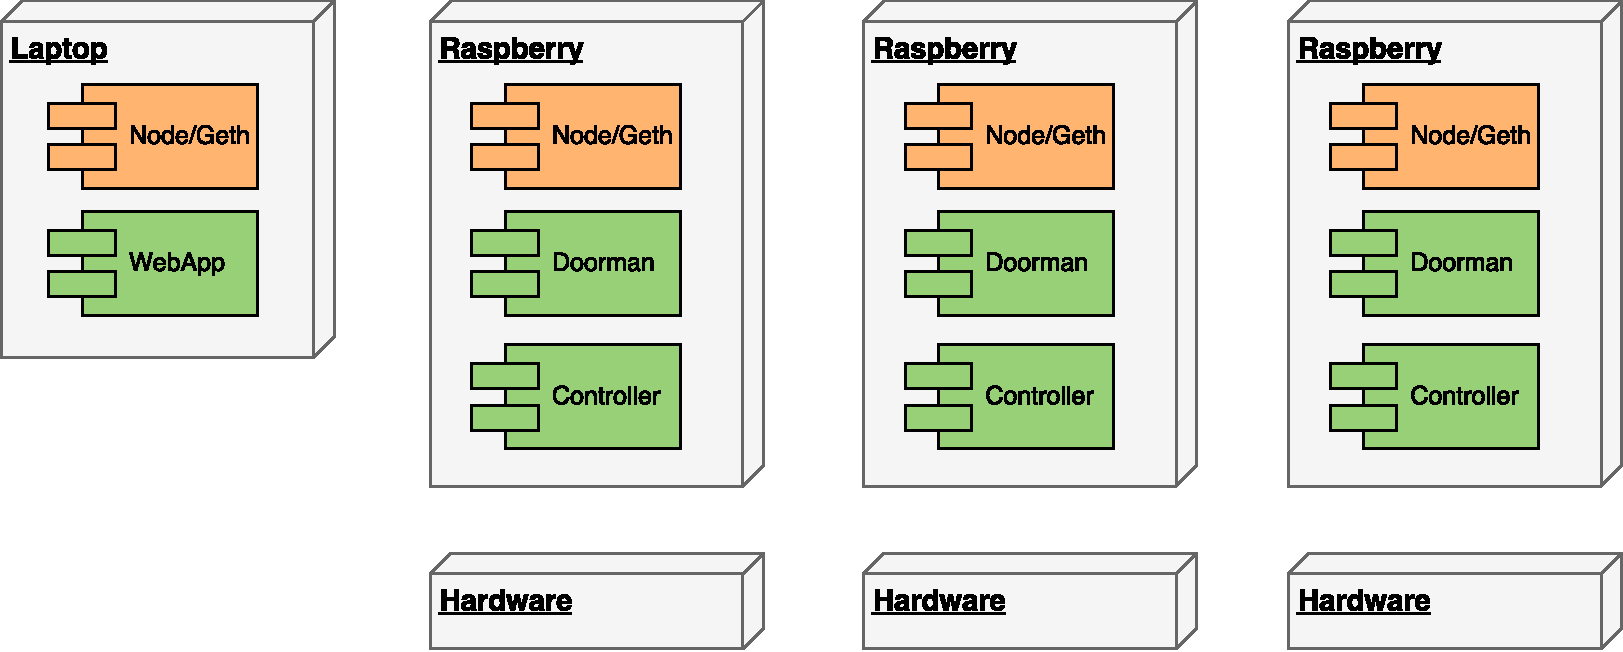
\includegraphics[width=.95\textwidth]{Aufbau_Komponenten} %{CS0031}
\caption{Komponenten und Schnittstellen}
\label{fig:Komponenten und Schnittstellen}
\end{figure}
\subsection{Systemkontext}

\subsection{Systemkomponenten}

\begin{figure}
\centering
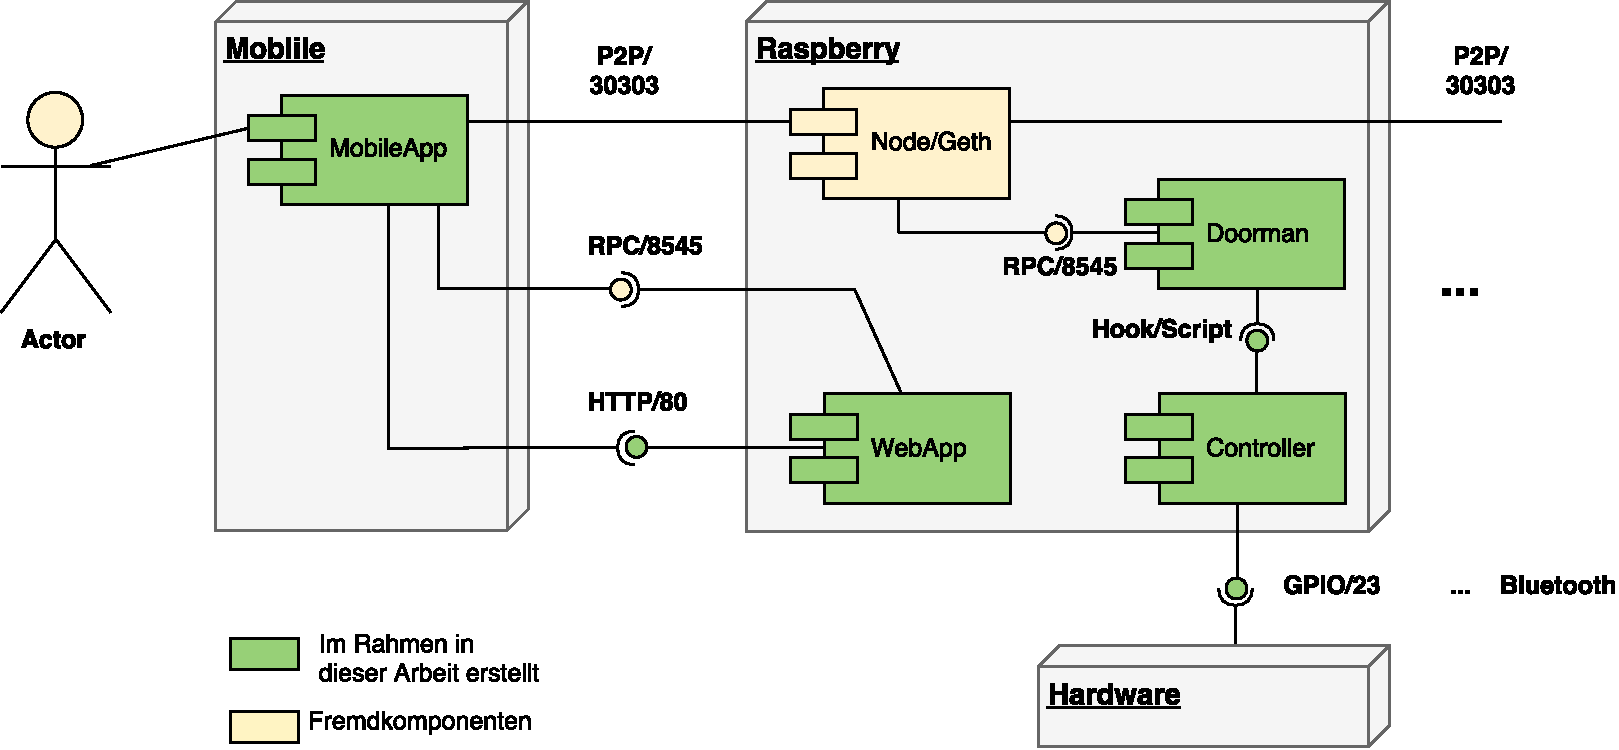
\includegraphics[width=.95\textwidth]{Aufbau_Komponenten_Interface} %{CS0031}
\caption{Komponenten und Schnittstellen}
\label{fig:Komponenten und Schnittstellen}
\end{figure}



\section{Blockchain}
\label{sec:Blockchain}
referenz, verweise

\subsection{Verwendete Implementation}
Wieso Ethereum?

\subsubsection{Ethereum}
\paragraph{Ledger?}
\paragraph{Solidity}
\paragraph{Whisper}
\subsubsection{IBM Hyperledger}
\paragraph{Fabric}
\paragraph{Chaintool}

\subsection{Testchain}

\subsection{Private chain mit Ethereum}


\subsection{Smart Contracts}
\label{subsec:Smart_Contracts}
\epigraph{''A computerized transaction protocol that executes the terms of a contract.``} \cite{BlockchainRevolution}
\\Mit diesem Zitat kann grob das Ziel von Smart Contracts beschrieben werden. Verträge, die in einem maschinenlesbaren Format verfasst sind, können mit unmissverständlicher Präzision und ohne Interpretationsspielraum definiert werden. So ist es möglich, einen deterministischen, digitalen Vertrag zu verfassen.
Entgegengesetzt ist es nahezu unmöglich eine Menge von Smart Contracts angesichts einer unüblichen Situation deterministisch abzuarbeiten. -> http://www.ibtimes.co.uk/pwc-blockchain-expert-pinpoints-sources-ambiguity-smart-contracts-1575778

\susubsection{Erstellen}
Um einen Smart Contract zu erstellen, wird mittels einer geeigneten Programmiersprache dieser formell definiert. Dieser geschriebene Programmcode kann mittels einer Transaktion in die Blockchain eingesetzt werden, wobei Initialwerte angegeben werden. Man sprich hierbei vom erstellen einer Instanz des Smart Contracts, ähnlich wie in der objektorientierten Programmierung. Bei der ausgelösten Transaktion gilt es zu beachten, dass diese keinen Empfänger hat; der Empfänger dieser Nachricht ist die Blockchain selbst. Wie bei jeder Transaktion eine gewisse Menge gas mitgegeben werden, damit die Operation abgeschlossen werden kann. Wenn der Code in die Blockchain eingesetzt wurde, erhält diese Instanz des Contracts eine Adresse, über die später mit dieser spezifischen Instanz interagiert werden kann.
Beim Erstellen eines Smart Contracts wird auch ein abi generiert. Dieses beschreibt die möglichen verfügbaren Attribute des Contracts und die Interaktionsmöglichkeiten (\#VGL. Funktionen) inklusive deren allfällige Parameter und Rückgabewerte (\#VGL. Interfacedeklaration in OO Sprachen).

\susubsection{Lesezugriff}
Um ein Attribut auszulesen oder eine Funktion mit konstantem Rückgabewert auszuführen, kann diese über ein verfügbares Interface, wie die JavaScript console von geth, direkt aufgerufen werden. Bei Funktionen mit konstantem Rückgabewert ist zu beachten, dass diese nur auf der lokalen Node emuliert werden (CITATION NEEDED) und es somit nicht möglich ist, eine Änderung in der Blockchain zu bewirken. Diese Funktionen haben folglich nur Lesezugriff.

\subsubsection{Schreibzugriff}
Wenn eine Funktion auf der Instanz aufgerufen wird, die eine Änderung in der Blockchain bewirkt, muss eine Transaktion ausgelöst werden. Der Sender der Transaktion muss dabei für die Kosten für gas und allfällige weitere Kosten (\#VGL. Bezahlbare Funktionen) aufkommen. Der Sender kann nicht nur ein Account sein, sondern auch ein weiterer Smart Contract, an dessen Adresse genügend Ether liegt, um die Transaktionskosten zu begleichen.

\paragraph{Bezahlbare Funktionen}
Einige Funktionen benötigen mehr Ether als nur die gas-Kosten. Wenn beispielsweise eine Dienstleistung oder Sache über einen Smart Contract verkauft werden soll, muss noch eine Menge Ether als Zahlungsmittel überweisen werden. Die Menge Ether ist im Smart Contract festgelegt und kann durch Inspektion des Programmcodes eingesehen werden. Sollte der Kunde zu wenig Ether schicken, kann der Smart Contract definieren, dass die Transaktion nicht erfolgreich ist und der Kunde sein Geld zurückerhält. Dazu kann die Transaktion selbst als nichtig erklärt werden und es muss nicht auf das Withdrawal Muster zuückgegriffen werden.

\subsubsection{Solidity}
Solidity ist eine Programmiersprache zur Erstellung von Smart Contracts auf der \acrfull{EVM}, die syntaktisch stark an JavaScript angelehnt ist. Sie kann auch auf anderen Blockchain Platoformen (wie Tendermint oder Counterparty für Bitcoin) verwendet werden. -> https://www.cryptocoinsnews.com/counterparty-brings-ethereum-smart-contracts-to-the-bitcoin-blockchain/\\Solidity wird, in Anlehnung auf den Ausdruck object-oriented, als contract-oriented beschrieben, da die erstellenden Konstrukte in der Sprache als ''contract`` und nicht ''object`` bezeichnet werden. Inhaltlich beziehen sich die beiden Ausdrücke auf dasselbe Konzept.

\subsubsection{Gängige Muster - GEHÖRT DAS INS KAPITEL "SMART CONTRACTS" ODER HIERHIN?}
Folgend werden einige Muster aufgelistet, die beim Entwurf und der Implementation von Smart Contracts mit Solidity, aufgrund der inhärenten Architektur der Platform und Sprache, beachtet werden sollten. Diese Muster dienen als Richtlinie und umgehen bekannte Limitationen oder schliessen Sicherheitslücken. Es ist möglich unter Misachtung der Muster Smart Contracts zu entwickeln. -> \#ALLE BEISPIELE VON http://solidity.readthedocs.io/en/develop/
\#Alle folgenden Beispiele waren für die Erarbeitung der Rentable \& RentableDiscovery Contracts zu beachten!

\paragraph{Generell}
Instanzen von Smart Contracts erhalten, wie Accounts, ebenfalls eine Adresse, an die Ether geschickt werden kann. Meistens wird dies in Form von Funktionsaufrufen gemacht, allerdings kann auch direkt an einen Smart Contract Ether überwiesen werden. Hierbei ist es wichtig zu beachten, dass der Ether zurückerstattet wird, der aus Veresehen an diesen gesendet wurde (\#VGL Withdrawal Muster).

\paragraph{Withdrawal Muster}
Wenn aus einem Smart Contract eine Transaktion an eine Adresse gestartet wird, muss das gas dafür vom digitalen Vertrag bezahlt werden (oder besser: vom Account, der die ursprüngliche Transaktion an den ersten digitalen Vertrag gestartet hat). Im Fall einer einfachen Überweisung fallen keine gas-Kosten an. Ist das Ziel aber ein anderer Smart Contract, besteht die Möglichkeit, dass der Zielvertrag Code ausführt, wenn er eine Transaktion erhält. Das Withdrawal Muster wird folglich verwendet, um zu verhindern, dass der Quellvertrag dies überprüfen muss oder für die gas-Kosten des anderen Smart contracts aufkommen muss.

Wird das Withdrawal Muster angewendet, überweist ein Smart Contract Ether nicht direkt an eine Zieladresse. Stattdessen merkt er sich die Menge, die einer Zieladresse zusteht und stellt die Möglichkeit zur Verfügung, dass diese Begünstigten Ether abheben können. Dies findet mittels einer Transaction statt, die vom Begünstigten ausgelöst werden muss. Die gas-Kosten für diese Art Funktionen sind meist vernachlässigbar und werden durch die zurückerhaltene Menge Ether kompensiert. Da der Begünstigte die Adresse des Quellvertrags kennt und den Quellcode von Smart Contracts öffentlich ist, kann die Zieladresse sicher gehen, beim aufrufen dieser withdrawal-Funktion auf dem Quellvertrag auch tatsächlich die Menge Ether zurückzuerhalten.
http://solidity.readthedocs.io/en/develop/common-patterns.html\#withdrawal-from-contracts

\#möglicherweise ein bildli zeichnen oder beispielcode einfügen


\paragraph{Re-Entrancy}
Hierbei handelt es sich um ein Muster, das angewendet wird, wenn in einem Smart Contract A ein interner Zustand existiert, der die Menge an Ether speichert, der \emph{anderen} zusteht und eine Möglichkeit besteht, diese Menge Ether zu entnehmen (\#VGL. Withdrawal Muster). Beispiele für zurückzuerstattenden Ether kann ein Gebot in einer Auktion sein oder Depots wie bei lokkit.
Unter der Annahme, dass die Zieladresse für die Rückerstattung ein Smart Contract B ist, kann B A angreifen. Bei einer Transaktion wird immer der zugehörige Code ausgeführt. Das heisst, dass B auf eine eingehende Transaktion reagieren kann und ihrerseits erneut die Transaktionsfunktion von A aktivieren kann (\#VGL. Withdrawal Muster). Wenn der Zustand von A noch nicht geändert wurde, wird der Betrag erneut gesendet, bis A kein Ether mehr zur Verfügung hat.

Um mehrfaches Überweisen von Ether zu verhindern, ist es essentiell, zuerst den internen Status des Vertrags zu ändern, bevor Ether überwiesen wird. Die \emph{total} zur Verfügung stehende Menge Ether eines Smart Contracts wird in der Blockchain gehalten und ist Teil des Konsensus. Es ist somit nicht möglich, dass mehr Ether ausgegeben wird als in dem jeweiligen digitalen Vertrag vorhanden ist. 

CODE SNIPPET FALSCH:
    function withdraw() {
        if (msg.sender.send(deposit[msg.sender])) { // das kann mehrere male ausgeführt werden.
            deposit[msg.sender] = 0;
        }
    }
CODE SNIPPET RICHTIG:
    function withdraw() {
        var currentRefund = deposit[msg.sender]; // zurückerstattend Menge auslesen
        deposit[msg.sender] = 0; // momentanes Depot zurücksetzen, bevor überwiesen wird! Dies wehrt die Re-Entrancy Attacke ab
        msg.sender.transfer(currentRefund); // hier transfer anstatt send benutzen, da (\#TODO)
    }

http://solidity.readthedocs.io/en/develop/security-considerations.html\#re-entrancy

\section{Komponenten}
\label{sec:Komponenten}
Nachfolgend werden die einzelnen Komponenten beschrieben, die für die volle Funktionalität der lokkit-Philosophie benötigt werden.
\subsection{Doorman}
Doorman implementiert die IoT-Seite der Benachrichtigungen mitterls Whisper Protokoll.
\subsubsection{Wieso Python? Wieso Python 2.7?}
\subsubsection{Mechanismus}

\subsection{Smart Contracts (Business Logik)}
Die Smart Contracts, die mit Solidity implementiert wurden, werden nachfolgend erläutert. Diese Smart Contracts bilden das Rückgrat der Applikation und bilden die Business Logik in Code Form ab und legen sich als Zugriffslayer zwischen die Userinteraktion und die Blockchain als Datenbank.

\#WICHTIG!!
Erwähnen der shortcomings, da unsere Contracts eine nicht vordefinierte Anzahl Iterationen haben. Dies kann aufgrund des Block-Gas limits zu stalling führen. Auch lese-Operationen, die aus anderen Smart-Contracts aufgerufen werden können diesen zum stallen bringen. -> http://solidity.readthedocs.io/en/develop/security-considerations.html\#gas-limit-and-loops

\subsubsection{Rentable}
\subsubsection{RentableDiscovery}

\subsubsection{Weitere Überlegungen}
noch einen separaten "data-store" für die Reservationen. Nicht-beachtete Konzepte. Raum für Verbesserungen.


\subsection{Frontend}
\subsubsection{Mobile App (Android)}
\paragraph{geth / offizielle API}
\paragraph{Status.io}
mit Verweis auf Testchain

\subsubsection{DApp}
\paragraph{Embark}
\paragraph{Vue.js}

\subsubsection{Command Line Client (geth attach)}


\section{}
\chapter{Schlussfolgerung}
\label{cha:Schlussfolgerung}

Abschliessend wird über das Projekt und dessen Ablauf reflektiert. Die erledigte Arbeit wird folgend infrage gestellt und eine kritische Position gegenüber der verwendeten Technologien, Entscheidungen im Projektverlauf und der Aufgabenstellung angenommen.

\section{Fazit Aufgabenstellung}
\label{sec:Fazit_Aufgabenstellung}
Die Umsetzung der erarbeiteten Aufgabenstellung dient als Demonstrator und soll ein \acrfull{PoC} sein. Der Fokus war von Anfang an, auch seitens der Auftraggebers, auf der Blockchain Technologie. Der \acrshort{IoT} Aspekt sollte der abschliessenden Veranschaulichung des \acrshort{PoC} dienen. Dabei gab es einige Limitationen in der Anwendung der Funktionalitäten der Blockchain, da auf die Komplexität und die Anwendungsbereiche der zu implementierenden Demonstrator Hardware Rücksicht genommen werden musste. Die physische Umsetzung des Demonstrators hat auch Zeit gekostet, die anders verwendet zu zusätzlichen Erkenntnissen im Bereich Blockchain hätte führen können.

Der unmittelbare Nutzen des Demonstrators, wo zentrale Angebote bereits vorhanden sind, beispielsweise an Bahnhöfen der SBB, ist nicht sofort ersichtlich. Einige Nachteile in diesem konkreten Beispiel wären benötigte Elektronik, Stromverbrauch und Verfügbarkeit des Angebots. Auch die Abhängigkeit zu der Blockchain kann verheerende Folgen haben, sollte dieses aus einem beliebigen Grund kompromittiert werden.

Das System wurde nur im Rahmen eines privaten Netzwerkes aufgebaut und getestet - kurze explorative Exkurse auf die \emph{Ropsten} Testchain sind davon ausgeschlossen. Skalierungsfragen wurden hierbei nicht beantwortet, wie beispielsweise die Performance und Zuverlässigkeit der Events aus Solidity oder Propagation von Whisper v5 Nachrichten in der öffentlichen Blockchain. Sollte erhebliche Latenz durch die Skalierung entstehen, wäre die Lösung so nicht zu verwenden und würde die Kundenzufriedenheit negativ beeinflussen.

\section{Fazit Blockchain}
Wie im Kapitel \ref{sec:Fazit_Aufgabenstellung} erwähnt, konnte aufgrund der Aufgabenstellung nicht alle Zeit in diesem Projekt in die Aufbereitung und Anwendung der Blockchain Technologie investiert werden. Trotzdem wurde ein Einblick in dieses Thema gewährt, der einen bleibenden Eindruck hinterliess.

Ein grosser Aspekt der Blockchain ist Anonymität und Vertrauenslosigkeit. Wie Schächen zu Stärken werden können, kann dies auch umgekehrt der Fall sein: Genau diese beiden Punkte werden zum Verhängnis, wenn konkrete Dienste angeboten werden sollen. An dieser Stelle sind Organisationen wie Silk Road\footnote{https://en.wikipedia.org/wiki/Silk\_Road\_(marketplace)} zu erwähnen, die im Angesicht solcher Technologien auf den Plan gerufen werden. Auch aufgrund des mangelnden Vertrauensverhältnisses zwischen Dienstleister und dem, der den Dienst bezieht, muss auf Vorsicht beharrt werden, falls Dienste in der realen Welt oder physische Produkte auf Bezahlung mit Kryptowährungen ausgetauscht werden.

\subsection{Fazit Ethereum}
Durch die Mitarbeit an dem Open Source Projekt go-ethereum wurde klar, dass das Ethereum Protokoll und auch die Umsetzung in geth trotz mehrjähriger Entwicklung noch lange keinen finalen Stand erreicht hat. Grundlegende Diskussion zum Design des Protokolls und dessen Implementation werden in den Kommunikationskanälen rege vorangetrieben.\cite[Gitter]{go-ethereum}

\section{Fazit Blockchain und IoT}
Das Konzept der Rentables wurde bewusst so abstrakt gewählt, um die Ausdehnung zu ermöglichen. Ein Rentable kann dabei grundsätzlich alles sein: Ein elektrisches Fahrrad, eine Ferienwohnung oder ein Schliessfach. Es muss jedoch möglich sein, einen Kontrollmechanismus anzubringen, der an eine Blockchain Node angebunden werden kann. Bei einem elektrischen Fahrrad wäre es z.B. möglich einen Minicomputer im Fahrgestellt zu montieren, welcher den Akku aktiviert oder deaktiviert und über eine Sim-Karte mit der Blockchain synchronisiert. Möchte ein Benutzer das Fahrrad verwenden, so müsste er dieses zuerst über die Blockchain mieten und erst dann kann er den Akku aktivieren. Die Mietkosten würden über den Smart Contract dem Anbieter des Fahrrades überwiesen werden.

\section{Ausblick}
Aufbauend auf diesem Demonstrator, dieser Arbeit und den Erkenntnissen daraus, könnte vom Auftraggeber Nutzen gezogen werden. Die weitere Verfolgung dieses Konzeptes könnte, unter Beachtung der weiteren Überlegungen im Bereich der Smart Contracts (vgl. \ref{para:Rentable_weitergehend}), verfeinert werden, und an Firmen demonstriert werden, um das noch vorhandene Mysterium um diese Smart Contracts in der Blockchain zu lüften.

\section{Lessons Learned}
\label{sec:Lessons_Learned}
Hier schreiben die Diplomanden ihre abschliessenden Worte zur Bachelorarbeit.

\subsection{Dominik Hirzel}
Das war das interessanteste und lehrreichste Projekt, an dem ich im schulischen und professionellen Umfeld je gearbeitet habe. Nie wollte ich mit einem meiner Kommilitonen tauschen. Diese Aussage dient nicht dazu, eine bessere Note ergaunern zu wollen, sondern soll vielmehr dazu meine Euphorie sowie meinen Arbeits- und Lernwillen in diesem Projekt auszudrücken. Einen grossen Teil dieser Motivation und Ausdauer verdanke ich auch meinem technisch wie sozial ausserordentlich versierten Partner: Andreas Schmid (vgl. \ref{andi}).

Die cutting edge Technologie der Blockchain interdisziplinär mit dem IoT Aspekt zu verbinden hat mir nicht nur schlaflose Nächte und eine Bekanntschaft mit dem Nachtwächter der HSLU beschert, sondern auch viele Freudensprünge erlaubt. Dieses Projekt hat mich in meiner Entscheidung bekräftigt, nach wie vor die passende Ausbildung und das passende Studium gewählt zu haben.

Speziell die Zusammenarbeit mit den Open Source Projekten Ethereum und Status-IM hat mir gefallen. Die Tatsache, dass wir ihnen in ihrem Design und der Implementation Fehler gefunden haben und diese mitteilen konnten (vgl. \ref{subsec:Open_Source}) bestätigt auch die Intensivität und unser Engagement in dieser Arbeit.

Die unterschiedlichen entworfenen Softwarekomponenten und das Zusammenspiel dieser, sowie das Design der Real-Time Kommunikationsschnittstelle und Berücksichtigung der Sicherheitsrelevanten Aspekte, waren aus technischer Sicht ein Highlight dieser Arbeit. Allgemein lässt sich die Komplexität dieses Systems betonen, das wir mit klar abgegrenzten Verantwortungsbereichen entworfen und umgesetzt haben.

\subsection{Andreas Schmid}
\label{andi}
Es bereitete mir Freude, mich mit meinem Kameraden in die weiten Abgründe der Blockchain und deren Smart Contracts zu stürzen. Gerade jetzt, wo das Thema brandaktuell ist und viele namhafte Firmen damit am Experimentieren sind, sind wir doch eines der ersten Teams, das einen funktionierenden und anfassbaren Demonstrator gebaut hat. Der Weg war holprig und nicht immer einfach und doch sind wir motiviert und erfolgreich am Ball geblieben. Herzlichen Dank an dieser Stelle an meinen kompetenten und ambitionierten Mitstreiter Dominik Hirzel.

Auch nach dieser sehr intensiven und aufregenden Zeit voller Überstunden und kurzen Nächten, ist mein Wissensdurst noch nicht gestillt und viele Fragen stehen noch offen. Diese Thematik wird mich sicherlich noch weiter beschäftigen.

Einmal mehr bin ich davon überzeugt, dass Open Source Projekte der richtige Ansatz für Software Engineering ist. Nur so kann die Zusammenarbeit über Projekte hinweg gefördert und weltbewegende Software geschrieben werden. Wir sind während dieser Arbeit stark in Kontakt mit den Entwicklern von Ethereum und Umsystemen geraten und haben sowohl für uns wie auch für die Community einen Nutzen generieren können.

Ich bin nach wie vor überzeugt, im richtigen Umfeld tätig zu sein und freue mich bereits auf die nächste Herausforderung. 


\include{chapters/09_Quellen_Tabellen_Abbildungsverzeichnisse}
%%%----------------------------------------------------------
%%%Anhang
\appendix
\chapter{Inhalt der CD-ROM/DVD}
\label{app:cdrom}

\paragraph{Format:} 
		CD-ROM, Single Layer, ISO9660-Format%


\section{PDF-Dateien}
\begin{FileList}{/}
\end{FileList}


\section{Sonstiges}

\begin{FileList}{/images}
\end{FileList}
	% Inhalt der CD-ROM/DVD

%%%----------------------------------------------------------
\MakeBibliography
%%%----------------------------------------------------------

%%%Messbox zur Druckkontrolle
\chapter*{Messbox zur Druckkontrolle}



\begin{center}
{\Large --- Druckgröße kontrollieren! ---}

\bigskip

\Messbox{100}{50} % Angabe der Breite/Hoehe in mm

\bigskip

{\Large --- Diese Seite nach dem Druck entfernen! ---}

\end{center}



\end{document}
